\section{Questão 1}
\subsection{A: Expressão para selecionar o material com menor peso}

A tensão de cisalhamento máxima no eixo cilíndrico é dada por:

\[
\tau_{\text{max}} = \frac{Tc}{J}
\]

Substituindo \( c = \frac{d}{2} \) e \( J = \frac{\pi d^4}{32} \):

\[
\tau_{\text{max}} = \frac{T \cdot \frac{d}{2}}{\frac{\pi d^4}{32}}
\]

Simplificando:

\[
\tau_{\text{max}} = \frac{T d}{2} \times \frac{32}{\pi d^4} = \frac{16T}{\pi d^3}
\]

Para minimizar o peso do eixo, consideramos a densidade do material \( \rho \) e o volume do eixo:

\[
\text{Massa} = \rho V = \rho \left(\frac{\pi d^2}{4} L\right)
\]

Substituindo \( d \) em função de \( \tau_{\text{ced}} \) (tensão de escoamento em cisalhamento):

\[
d = \left(\frac{16T}{\pi \tau_{\text{ced}}}\right)^{1/3}
\]

A massa do eixo fica:

\[
\text{Massa} = \rho L \frac{\pi}{4} \left(\frac{16T}{\pi \tau_{\text{ced}}}\right)^{2/3}
\]

Para minimizar a massa, precisamos maximizar o \textit{índice de seleção} \( M \), que é a relação entre a tensão de escoamento e a densidade

\[
M = \frac{\tau_{\text{ced}}^{2/3}}{\rho}
\]

\subsection{Questão (b): Selecionar os 4 melhores materiais}

\begin{figure}[h]
    \centering
    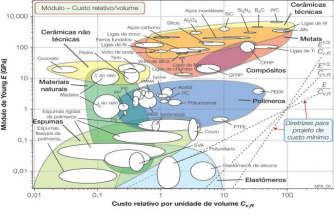
\includegraphics[width=.7\linewidth]{grafico tensao}
    \caption{Gráfico de tensão de escoamento em função da densidade}
\end{figure}

Com base no gráfico fornecido, devemos selecionar os materiais com maior \( M = \frac{\tau_{\text{ced}}^{2/3}}{\rho} \).

No gráfico, os materiais mais à esquerda e acima das retas de declive 1.5 são os melhores. Os quatro melhores parecem ser:

\begin{itemize}
    \item Ligas endurecíveis de alumínio ("Age-hardening wrought Al-alloys")
    \item Ligas de magnésio ("Wrought magnesium alloys")
    \item Ligas de titânio ("Titanium alloys")
    \item Compósitos CFRP (Carbon Fiber Reinforced Polymer, com matriz epóxi isotrópica)
\end{itemize}

Esses materiais apresentam boa resistência ao cisalhamento e baixa densidade.

\section{Prática 2: Sobre diagrama de propriedade}

\subsection{(a) Material mais próximo da reta de inclinação 1.5}

A reta de inclinação 1.5 passa pelo ponto \( \rho = 100 \) kg/m³ e \( \tau_{\text{ced}} = 10 \) MPa.

No gráfico, um dos materiais mais próximos dessa reta é **Softwood: pine, along grain (madeira de pinho ao longo do grão)**.

\subsection{(b) Dispersão na densidade dos materiais como madeira e cortiça}

Materiais naturais, como **madeiras e cortiça**, apresentam maior dispersão na densidade porque sua estrutura é **heterogênea**, variando conforme:

\begin{itemize}
    \item **Localização da árvore** (região climática, tipo de solo)
    \item **Processamento** (umidade, compactação)
    \item **Variação estrutural** (madeira pode ter mais ou menos fibras celulósicas)
\end{itemize}

Já materiais como **Teflon e Nylon** são **polímeros sintéticos**, produzidos industrialmente com controle rigoroso de composição e processamento, resultando em menor variação na densidade.

\subsection{(c) Dispersão da tensão de escoamento em metais puros}

Metais puros, como **cobre (Copper), estanho (Tin) e chumbo (Lead)**, apresentam grande dispersão na tensão de escoamento devido a:

\begin{itemize}
    \item **Impurezas**: pequenas variações na composição química afetam a resistência.
    \item **Processamento**: a tensão pode mudar dependendo se o metal é recozido (mole) ou encruado (duro).
    \item **Granulação e microestrutura**: quanto menores os grãos, maior a resistência.
\end{itemize}

Isso faz com que haja uma ampla faixa de resistência mecânica para esses metais no gráfico.

\subsection{(d) Diferença entre ligas "cast" e "wrought"}

\begin{itemize}
    \item **"Cast" (fundidas)** → Produzidas por **fusão e solidificação** em moldes. Têm boa conformabilidade, mas são menos resistentes mecanicamente devido à presença de porosidade.
    \item **"Wrought" (forjadas/trabalhadas)** → São **laminadas, extrudadas ou forjadas**, resultando em melhor resistência mecânica e menor presença de defeitos internos.
\end{itemize}

Em português, chamamos:

\begin{itemize}
    \item **"Cast alloys"** = Ligas fundidas
    \item **"Wrought alloys"** = Ligas trabalhadas ou forjadas
\end{itemize}

\section{Resumo das Respostas}

\begin{enumerate}
    \item **Expressão para minimizar peso** → Maximizar \( M = \frac{\tau_{\text{ced}}^{2/3}}{\rho} \).
    \item **4 melhores materiais** → Ligas de alumínio endurecíveis, magnésio, titânio e compósitos CFRP.
    \item **Material mais próximo da reta de inclinação 1.5** → **Madeira de pinho (Softwood: pine, along grain)**.
    \item **Variação na densidade de materiais naturais** → Estrutura heterogênea e variações ambientais.
    \item **Dispersão na resistência de metais puros** → Impurezas, processamento e microestrutura.
    \item **Diferença entre "cast" e "wrought"** → Fundidas (moldadas) vs. forjadas (trabalhadas mecanicamente).
\end{enumerate}
